% Chapter 9: Análisis de Riesgo
\chapter{Análisis de Riesgo}

\section{Identificación y Mitigación de Riesgos Sistémicos}

La consultoría en ingeniería minera está expuesta tanto a la volatilidad macroeconómica del ciclo de materias primas como a complejidades operacionales específicas de su cartera de proyectos.

\begin{figure}[htbp]
\centering
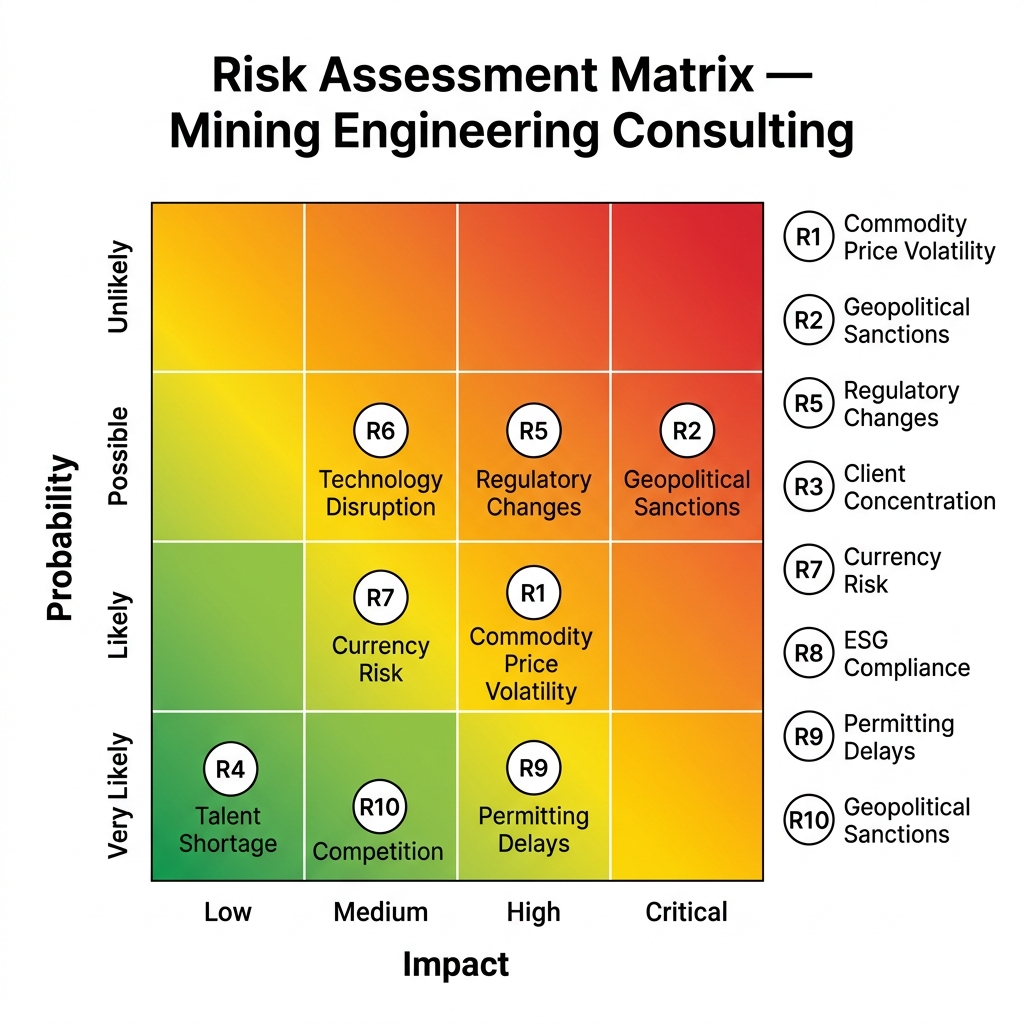
\includegraphics[width=0.88\textwidth]{../figures/05_risk_heatmap.png}
\caption{Matriz de Evaluación de Riesgos para la Consultoría de Ingeniería Minera.}
\label{fig:risk_map}
\end{figure}

A continuación se detallan los 5 riesgos de mayor impacto para REDCO y sus estrategias de mitigación:

\begin{enumerate}
    \item \textbf{R2 - Sanciones Geopolíticas y Concentración en Rusia (Efecto Seligdar):}
    \begin{itemize}
        \item \textbf{Impacto:} Crítico | \textbf{Probabilidad:} Posible.
        \item \textbf{Descripción:} Bloqueo de pagos, imposibilidad de exportar software/servicios de ingeniería a operadores sancionados (Polyus, Seligdar), daño reputacional.
        \item \textbf{Mitigación:} Activación del escenario base ajustado en flujo de caja (ignorar ingresos POM de Rusia para financiamiento operacional). Canalizar cualquier servicio remanente vía intermediarios en Asia Central o China que actúen como buffer legal.
    \end{itemize}

    \item \textbf{R3 - Concentración de Clientes:}
    \begin{itemize}
        \item \textbf{Impacto:} Alto | \textbf{Probabilidad:} Likely.
        \item \textbf{Descripción:} Dependencia de 1 o 2 grandes proyectos o clientes (p.ej., REDCO dependiendo excesivamente del POM ruso o de un único operador en Chile).
        \item \textbf{Mitigación:} Diversificación comercial agresiva hacia Perú y Brasil. Establecer un límite máximo de exposición de facturación por cliente del 25\%.
    \end{itemize}

    \item \textbf{R4 - Escasez de Talento Clave:}
    \begin{itemize}
        \item \textbf{Impacto:} Medio | \textbf{Probabilidad:} Very Likely.
        \item \textbf{Descripción:} Dificultad para reclutar y retener ingenieros de procesos, planificadores mineros y geotecnistas de alto nivel frente a las ofertas de operadores mineros directos.
        \item \textbf{Mitigación:} Desarrollar el baseline organizacional de REDCO (Pilar B - Capability × Personal Identity) para estructurar planes de carrera, flexibilidad laboral y bonos por desempeño alineados al margen de proyectos.
    \end{itemize}

    \item \textbf{R9 - Retrasos en Permitting de Proyectos de Clientes:}
    \begin{itemize}
        \item \textbf{Impacto:} Alto | \textbf{Probabilidad:} Very Likely.
        \item \textbf{Descripción:} Los clientes congelan la ingeniería de detalle porque sus EIAs están atrapados en el SEA (Chile) o Senace (Perú).
        \item \textbf{Mitigación:} Desarrollar capacidades internas de pre-permitting e ingeniería regulatoria para integrarlas en etapas tempranas y ayudar al cliente a acelerar la obtención de permisos.
    \end{itemize}

    \item \textbf{R1 - Volatilidad del Precio de los Metales:}
    \begin{itemize}
        \item \textbf{Impacto:} Alto | \textbf{Probabilidad:} Likely.
        \item \textbf{Descripción:} Caída drástica del cobre o hierro reduce el CAPEX de los clientes, cancelando proyectos de ingeniería.
        \item \textbf{Mitigación:} Pivotar la propuesta de valor en periodos de precios bajos hacia OPEX (ingeniería de optimización de costos, eficiencia hídrica y de procesos operacionales) que las mineras contratan activamente para mantener márgenes.
    \end{itemize}
\end{enumerate}
